\documentclass[preview]{standalone}

\usepackage{amsmath}
\usepackage{amssymb}
\usepackage{parskip}
\usepackage{fullpage}
\usepackage{tikz}
\usepackage{hyperref}
\usepackage{stellar}
\usepackage{definitions}

\begin{document}

\id{euleridentity}
\genpage

\section{Euler's Formula}

\begin{snippettheorem}{euler-formula}{Euler's Formula}
    Euler's formula states that for every \(x\in\mathbb{R}\)
    \begin{align*}
        e^{ix}=\cos(x)+i\sin(x)
    \end{align*}
\end{snippettheorem}

\begin{snippet}{euler-formula-illustration}
We can represent Euler's formula on the complex plane

\begin{center}
    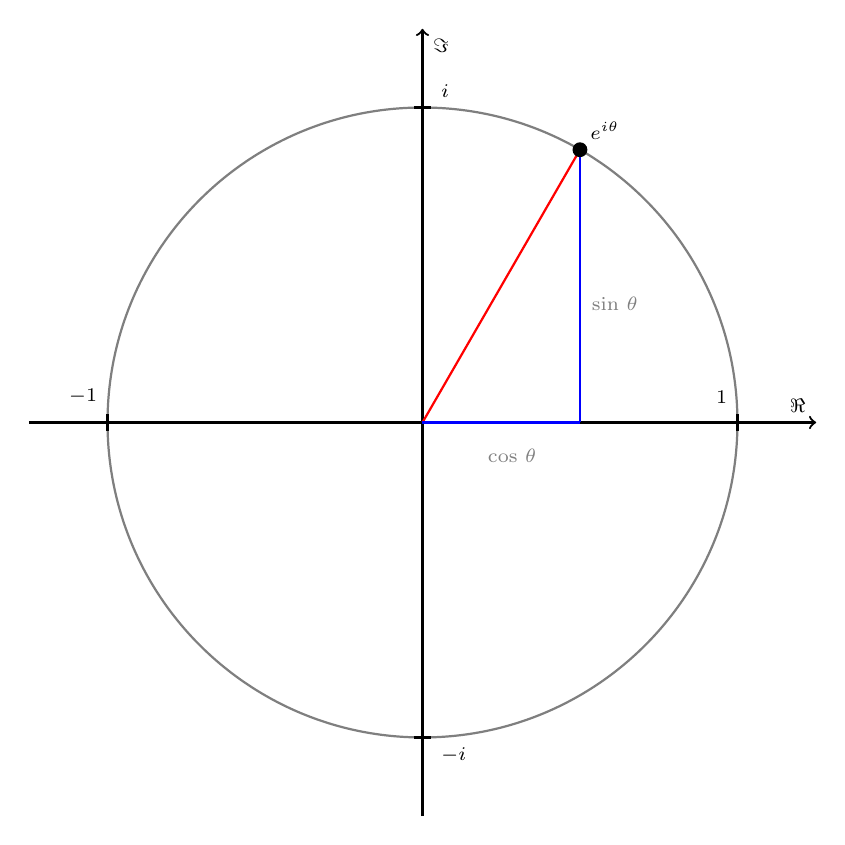
\begin{tikzpicture}
        \begin{scope}[thick, font=\scriptsize, scale=4]
            \draw [->] (-1.25,0) -- (1.25,0) node [above left]  {\(\Re\)};
            \draw [->] (0,-1.25) -- (0,1.25) node [below right] {\(\Im\)};
        
            \draw (1,-0.75pt) -- (1,0.75pt)   node [above left] {\(1\)};
            \draw (-1,-0.75pt) -- (-1,0.75pt) node [above left] {\(-1\)};
            \draw (-0.75pt,1) -- (0.75pt,1)   node [above right] {\(i\)};
            \draw (-0.75pt,-1) -- (0.75pt,-1) node [below right] {\(-i\)};

            \path [draw=black,fill=none,semitransparent] (0, 0) circle (1);
            \draw [thick, color=red] (0,0) -- (0.5,0.866);
            \draw [thick, color=blue] (0.5,0) -- (0.5,0.866);
            \draw [thick, color=blue] (0,0) -- (0.5,0);
            
            \draw [color=black, fill=black] (0.5,0.866) circle(0.02) node [above right] {\(e^{i\theta}\)};
            
            \node [below right,gray] at (0.175, -0.05) {\(\cos\,\theta\)};
            \node [below right,gray] at (0.505, 0.43) {\(\sin\,\theta\)};
        \end{scope}
    \end{tikzpicture}
\end{center}

We can notice that \(\left|e^{ix}\right|=1\) since \(|e^{i\theta}|=\cos^2\theta +\sin^2\theta =1\)
\end{snippet}

\section{Proof}

\begin{snippet}{euler-formula-proof-expl1}
To understand this identity we must first look at the Taylor series of some functions.
These functions are all equal to their Taylor series, so we can easily compute their Maclaurin series.
\end{snippet}

\subsection{Exponential function}

\begin{snippetproposition}{exponential-function-taylor-series}{Exponential Function Taylor Series}
    The Taylor series of \(e^x\) is given by
    \[
        e^x=\sum_{n=0}^{\infty}\frac{x^n}{n!}
    \]
\end{snippetproposition}

\begin{snippetproof}{exponential-function-taylor-series-proof}{Exponential Function Taylor Series}
    The first thing we can notice is that the derivative of \(f(x)=e^x\) is \(e^x\) itself, so
    \begin{align*}
        f^{(n)}(x)=e^x,
        \quad n\in\mathbb{Z}
    \end{align*}
    which means that for every term of the Maclaurin series
    \begin{align*}
        f^{(n)}(a)=f^{(n)}(0)=e^0=1
    \end{align*}
    The exponential function can then be expressed as the series
    \begin{align*}
        e^x=\sum_{n=0}^{\infty}\frac{x^n}{n!}
    \end{align*}
\end{snippetproof}

\subsection{Sine function}

\begin{snippetproposition}{sine-function-taylor-series}{Sine Function Taylor Series}
    The Taylor series of \(\sin(x)\) is given by
    \[
        \sin(x)=\sum_{n=0}^{\infty}\frac{x^{2n+1}{(-1)}^n}{(2n+1)!}
    \]
\end{snippetproposition}

\begin{snippetproof}{sine-function-taylor-series-proof}{Sine Function Taylor Series}
    Here's a table of the derivatives of \(f(x)=\sin(x)\) and their value at \(a=0\)
    \begin{align*}
        \begin{cases}
            f^{(0)}(x)=\sin(x), \quad &f^{(0)}(0)=0 \\
            f^{(1)}(x)=\cos(x), \quad &f^{(1)}(0)=1 \\
            f^{(2)}(x)=-\sin(x),\quad &f^{(2)}(0)=0 \\
            f^{(3)}(x)=-\cos(x),\quad &f^{(3)}(0)=-1\\
        \end{cases}
    \end{align*}
    The next derivative is \(f^{(4)}(x)=\sin(x)\) making the sequence start over.
    \\
    We can notice that every even n-th derivative will multiply the term by \(0\).
    \\
    We will use \(2n+1\) to skip all the even integers.
    \\
    We can also notice that the sign of the term is given by \({(-1)}^n\) since we only consider odd indexes.
    \begin{align*}
        \sin(x)&=x-\frac{x^3}{3!}+\frac{x^5}{5!}-\frac{x^7}{7!}+\cdots
        \\
        &=\sum_{n=0}^{\infty}\frac{x^{2n+1}{(-1)}^n}{(2n+1)!}
    \end{align*}
\end{snippetproof}

\subsection{Cosine function}

\begin{snippetproposition}{cosine-function-taylor-series}{Cosine Function Taylor Series}
    The Taylor series of \(\cos(x)\) is given by
    \[
        \cos(x)=\sum_{n=0}^{\infty}\frac{x^{2n}{(-1)}^n}{(2n)!}
    \]
\end{snippetproposition}

\begin{snippetproof}{cosine-function-taylor-series-proof}{Cosine Function Taylor Series}
    Here's a table of the derivatives of \(f(x)=\cos(x)\) and their value at \(a=0\)
    \begin{align*}
        \begin{cases}
            f^{(0)}(x)=\cos(x), \quad &f^{(0)}(0)=1 \\
            f^{(1)}(x)=-\sin(x),\quad &f^{(1)}(0)=0 \\
            f^{(2)}(x)=-\cos(x),\quad &f^{(2)}(0)=-1\\
            f^{(3)}(x)=\sin(x), \quad &f^{(3)}(0)=0 \\
        \end{cases}
    \end{align*}
    The next derivative is \(f^{(4)}(x)=\cos(x)\) making the sequence start over.
    \\
    We can notice that every odd n-th derivative will multiply the term by \(0\).
    \\
    We will use \(2n\) to skip all the odd integers.
    \\
    We can also notice that the sign of the term is given by \({(-1)}^n\) since we only consider even indexes.
    \begin{align*}
        \cos(x)&=1-\frac{x^2}{2!}+\frac{x^4}{4!}-\frac{x^6}{6!}+\cdots
        \\
        &=\sum_{n=0}^{\infty}\frac{x^{2n}{(-1)}^n}{(2n)!}
    \end{align*}
\end{snippetproof}

\subsection{Conclusion}

\begin{snippetproof}{euler-formula-proof}{Euler's Formula}
    Given the Taylor series for the exponential function
    \begin{align*}
        e^x=\sum_{n=0}^{\infty}\frac{x^n}{n!}
    \end{align*}
    we use \(ix\) instead of \(x\)
    \begin{align*}
        e^{ix}=\sum_{n=0}^{\infty}\frac{{(ix)}^n}{n!}
    \end{align*}
    Consider the exponentiation table of \(i\).
    \begin{align*}
        \begin{cases}
            i^0=+1\\
            i^1=+i\\
            i^2=-1\\
            i^3=-i\\
        \end{cases}
        \quad
        \begin{cases}
            i^4=+1\\
            i^5=+i\\
            i^6=-1\\
            i^7=-i\\
        \end{cases}
        \quad
        \cdots
    \end{align*}
    We can use these properties to simplify the \(e^{ix}\) Taylor series
    \begin{align*}
        e^{ix}
        &   =1
            +ix
            +\frac{{(ix)}^2}{2!}
            +\frac{{(ix)}^3}{3!}
            +\frac{{(ix)}^4}{4!}
            +\frac{{(ix)}^5}{5!}
            +\frac{{(ix)}^6}{6!}
            +\frac{{(ix)}^7}{7!}
            +\cdots
        \\
        \\
        &   =1
            +ix
            -\frac{x^2}{2!}
            -\frac{ix^3}{3!}
            +\frac{x^4}{4!}
            +\frac{ix^5}{5!}
            -\frac{x^6}{6!}
            -\frac{ix^7}{7!}
            +\cdots
        \\
        \\
        &=
        \left(
            1
            -\frac{x^2}{2!}
            +\frac{x^4}{4!}
            -\frac{x^6}{6!}
            +\cdots
        \right)
        +i
        \left(
            x
            -\frac{x^3}{3!}
            +\frac{x^5}{5!}
            -\frac{x^7}{7!}
            +\cdots
        \right)
    \end{align*}
    We notice that the two terms correspond to the sine and cosine Taylor series
    \begin{align*}
        e^{ix}=\cos\,x+i\,\sin\,x
    \end{align*}
\end{snippetproof}

\section{Complex trigonometric functions}

\begin{snippetdefinition}{complex-sine-definition}{Complex Sine}
    By the Euler identify we can define \(\sin(x)\) for \(x \in \mathbb{C}\) as
    \[ \sin(x)=\frac{e^{ix}+e^{-ix}}{2i} \]
\end{snippetdefinition}

\begin{snippetdefinition}{complex-cosine-definition}{Complex Cosine}
    By the Euler identify we can define \(\cos(x)\) for \(x \in \mathbb{C}\) as
    \[ \cos(x)=\frac{e^{ix}-e^{-ix}}{2} \]
\end{snippetdefinition}

\end{document}